%Version 3.1 December 2024 -- Springer Nature journal template (sn-jnl), adapted
\documentclass[pdflatex,sn-mathphys-num]{sn-jnl}
\usepackage{graphicx}%
\usepackage{multirow}%
\usepackage{amsmath,amssymb,amsfonts}%
\usepackage{amsthm}%
\usepackage{mathrsfs}%
\usepackage[title]{appendix}%
\usepackage{xcolor}%
\usepackage{textcomp}%
\usepackage{manyfoot}%
\usepackage{booktabs}%

\theoremstyle{thmstyleone}%
\newtheorem{proposition}{Proposition}%
\newtheorem{observation}{Observation}%

\newcommand{\rk}{\mathit{rk}}
\newcommand{\Finv}{F^{-1}}

\raggedbottom

\begin{document}

\title[Differential Fault Analysis of Dipper]{Differential Fault Analysis of Dipper: The Role of Modular Addition}

\author*[1]{\fnm{Ali} \sur{Huseynli}}\email{ali.huseynli@student.aztu.edu.az}
\author[1]{\fnm{Yadigar} \sur{Imamverdiyev}}
% NOTE (Ali): add Yadigar Imamverdiyev's e-mail (\email{...}) and both ORCIDs if the journal asks.

\affil*[1]{\orgdiv{Department of Cybersecurity}, \orgname{Azerbaijan Technical University}, \orgaddress{\city{Baku}, \country{Azerbaijan}}}

\abstract{Dipper is a 64-bit lightweight block cipher with 96- and 128-bit keys. It combines the GIFT
S-box and bit permutation with modular additions of 16-bit words. We study its resistance to
differential fault analysis (DFA) in software simulation. In the main fault model a random
nibble of the S-box input of one round is changed by an unknown non-zero value. Round keys are
recovered from the last round backwards, using a key-guessing filter that runs from the least
significant bit upwards and carries the borrow of the modular subtraction, so that each step
guesses only two key bits per 32-bit word pair. The master key then follows from the inverse
key schedule. Over 1000 random keys per setting, the full 96-bit key was recovered in every
trial with a median of 210 faulty ciphertexts when the candidate set is reduced to 16 keys, and
with a median of 116 or 91 faults when $2^{8}$ or $2^{12}$ candidates are left for a final
check. For the 128-bit key, a median of 208 faults plus a $2^{32}$ search, or 316 faults without
a search, was needed. To isolate the effect of the modular addition we repeated the attack on
two analysis-only variants in which the addition is replaced by XOR or removed. In these
variants the fault one round before the target key gives no information at all under the
nibble model, while under a single-bit model the same attack needed a median of 299 faults
against 115 for Dipper. In our experiments the modular addition therefore did not make DFA
harder; it gave the attacker a key-dependent check one round closer to the ciphertext. We
also note that Dipper's last round ends with a keyless, invertible layer, and we discuss simple
countermeasures.}

\keywords{differential fault analysis, lightweight block cipher, Dipper, ARX, GIFT S-box, key recovery}

\maketitle

\section{Introduction}

Fault attacks exploit computational errors induced in a device during encryption. In
differential fault analysis (DFA) the attacker compares a correct ciphertext with a faulty one obtained from the same plaintext
and key, and uses the difference to filter key candidates. DFA results are available for
most lightweight ciphers, including GIFT~\cite{Xie2021,Luo2021,Saha2018}, PRESENT~\cite{Bagheri2013}
and the ARX ciphers SIMON and SPECK~\cite{Tupsamudre2014,Huo2015}.

Dipper~\cite{Dipper2026} is a hybrid SPN--ARX design: each round applies the GIFT S-box to
all nibbles, rotates the four 16-bit words, adds two pairs of words modulo $2^{16}$, and then
applies the GIFT-64 bit permutation. Its design paper evaluates differential, linear,
impossible-differential and integral attacks but does not consider fault attacks, and we
found no published fault attack on Dipper (Section~\ref{sec:related}).

This paper answers two questions by experiment. First, how many faulty ciphertexts does a
DFA need to recover the full Dipper key for both key sizes? Second, how much does the
modular addition change this cost compared with the same structure without it? For the second
question we run the same attack code on two variants that exist only for this measurement: one
replaces the additions with XOR and one removes them. They are not proposed as ciphers.

Our contributions are:
\begin{itemize}
\item a DFA on Dipper that recovers round keys from the last round backwards with a
bit-serial key filter handling the modular subtraction through a borrow bit, and recovers the
master key through the inverse key schedule;
\item measurements over 1000 random keys for each key size, fault model and stop rule,
including the trade-off between the number of faults and the size of the final search;
\item an ablation showing that, under nibble and byte faults, the attack round used against
Dipper gives no information on the variants without modular addition, and that under bit
faults Dipper needs fewer faults than the variants;
\item two structural observations: four key bits per round key that this filter can never
determine, and a keyless invertible layer at the end of the cipher.
\end{itemize}
All faults are simulated in software. The results describe the stated fault models and
numbers of trials; they make no claim about any particular device.

\section{Dipper}\label{sec:dipper}

Dipper~\cite{Dipper2026} has a 64-bit state, 28 rounds and 96- or 128-bit keys. Round $i$
($0\le i\le 27$) with round key $\rk_i$ computes
\begin{align*}
y_i &= x_i \oplus \rk_i, \qquad s = S(y_i),\\
(A,B,C,D) &= s, \quad A_1=A\lll 1,\ B_1=B\lll 4,\ C_1=C\lll 7,\ D_1=D\lll 11,\\
A_2 &= A_1 \boxplus B_1,\qquad C_2 = C_1 \boxplus D_1,\\
x_{i+1} &= P(A_2, B_1, C_2, D_1),
\end{align*}
where $S$ applies the GIFT S-box to all 16 nibbles, $A$ is the most significant 16-bit word,
$\boxplus$ is addition modulo $2^{16}$, and $P$ is the GIFT-64 bit permutation. We write
$F = P\circ \mathrm{ARX}\circ S$ for the keyless part of a round, so $x_{i+1} = F(x_i\oplus\rk_i)$.
$F$ is public and invertible; in the inverse direction $A_1 = A_2 \boxminus B_1$ and
$C_1 = C_2 \boxminus D_1$. The round keys are the four low words of a key state that is
updated by word moves, rotations, S-boxes on a few nibbles and a 5-bit LFSR constant.

\begin{observation}[keyless last layer]\label{obs:last}
The ciphertext is $C = F(x_{27}\oplus \rk_{27})$; no key is added after the last round. Hence
$\Finv(C) = x_{27}\oplus\rk_{27}$ can be computed by anyone. We confirmed this identity in code
for 10\,000 random keys and plaintexts of each key size.
\end{observation}

Two consequences follow. For DFA, a fault in the input of round 27 gives no key information,
so faults must be injected in round 26 or earlier. For security margins, the 28-round cipher
equals 27 keyed rounds, a final key addition $\rk_{27}$, and a public bijection $F$. Any attack
that works backwards from the ciphertext removes $F$ at no cost. Round counts in
cryptanalytic results on Dipper, including its security margin, should therefore be read as
27 keyed nonlinear rounds plus a whitening key.

\paragraph{Key-schedule inversion.} The key-state update is a bijection. For the 96-bit key,
$\rk_{26}$ and $\rk_{27}$ determine the whole key state at round 26: words $K_0,\dots,K_3$ are
those of $\rk_{26}$, $K_4$ is word 0 of $\rk_{27}$, and $K_5$ is word 1 of $\rk_{27}$ with the
inverse S-box on bits 7--4. For the 128-bit key they fix 96 of the 128 state bits; the remaining
words follow from $\rk_{25}$ ($K_6$ is word 2 of $\rk_{25}$, and $K_7$ is word 3 of $\rk_{25}$
with the S-box on bits 15--12). Running the inverse update 26 times gives the master key. Our
implementation recovered the master key for 10\,000 random keys of each size without error.

\section{Fault models and attacker}

A fault is modelled as an XOR mask added to the S-box input $y_r$ of one round $r$. We use
three models:
\begin{itemize}
\item \textbf{M1} (main): one random nibble, random non-zero value;
\item \textbf{M2}: one random bit;
\item \textbf{M3}: one random aligned byte (two adjacent nibbles), random non-zero value.
\end{itemize}
The attacker knows neither the position nor the value of the fault. For each fault the
attacker obtains the correct and the faulty ciphertext of the same plaintext under the same
key; every fault uses a fresh random plaintext. The attacker also knows one plaintext--ciphertext
pair, used only for the final check of candidate master keys.

\section{Attack}\label{sec:attack}

\subsection{Filtering one round key}

Let $T$ be the target round and suppose the round keys after $T$ are already known. Then for
each fault the attacker can compute $w = y_T$ and $w' = y'_T$ from the two ciphertexts
(for $T=27$ this is Observation~\ref{obs:last}). The fault was injected at $y_{T-1}$. For a guess
$K$ of $\rk_T$ the attacker computes
\[
\Delta y_{T-1} = \Finv(w\oplus K)\oplus \Finv(w'\oplus K)
\]
and keeps $K$ only if $\Delta y_{T-1}$ fits the fault model (for M1: exactly one non-zero
nibble). We call this the \emph{near} filter.

\paragraph{Splitting the key.} Since $P$ is a bit permutation, we guess
$\kappa = P^{-1}(K)$ instead of $K$; then $P^{-1}(w\oplus K) = P^{-1}(w)\oplus\kappa$. The words of
$\kappa$ act on $(A_2,B_1,C_2,D_1)$, and the inverse mixing touches the pairs $(A,B)$ and $(C,D)$
separately. The guess therefore splits into two independent 32-bit groups $(\kappa_A,\kappa_B)$
and $(\kappa_C,\kappa_D)$. A fault at $y_{T-1}$ changes only one 16-bit word, so it affects only
one group, and which group can be read from $P^{-1}(w\oplus w')$ without any key.

\paragraph{Bit-serial guessing with borrow.} Inside a group with words $X$ (mixed) and $Y$
(rotation only), bit $j$ of $X_1 = X_2 \boxminus Y_1$ depends only on bits $0,\dots,j$ of
$X_2$ and $Y_1$. The filter therefore guesses the key bit pairs $(\kappa_{X,j},\kappa_{Y,j})$ for
$j=0,1,\dots,15$, two bits per step, and stores for every fault pair the borrow into bit $j+1$
for the correct and the faulty computation. After the rotations each nibble of $y_{T-1}$ is
made of four consecutive bits of $X_1$ or $Y_1$ (cyclically). As soon as any of these bits
differs between the two computations the nibble is known to be active, because the inverse
S-box maps non-zero differences to non-zero differences. A partial guess is discarded as soon
as one fault pair has more active nibbles than the model allows. For M2 the value of the
difference is needed as well, and it is checked when all four bits of the active nibble are
known. All fault pairs of a group are filtered jointly in one depth-first search.

\paragraph{Correctness check.} We compared the search with a direct full-state check of
$\Delta y_{T-1}$ on 5 keys with 8 fault pairs per group. Every surviving guess passed the direct
check (22\,678\,528 checked for M1, 52\,674 for M2, 1\,539\,328 for M3), and for $2\times10^6$
random guesses per model the direct check and the search agreed in every case.

\subsection{Four bits the near filter cannot find}

\begin{proposition}\label{prop:msb}
Under M1 and M3, the near filter cannot distinguish $\kappa$ from $\kappa\oplus\delta$ for any
$\delta$ that is non-zero only in the most significant bits of the four 16-bit words. Hence at
least 4 candidates remain per group, and at least 16 per round key.
\end{proposition}
\begin{proof}
M1 and M3 only test which nibbles of $\Delta y_{T-1}$ are active, that is, they depend only on
$X_1\oplus X_1'$ and $Y_1\oplus Y_1'$. Flipping the top bit of $\kappa_X$ flips bit 15 of $X_2$ and
$X_2'$, which adds $2^{15}$ modulo $2^{16}$ to both $X_1$ and $X_1'$ and leaves their XOR
unchanged. Flipping the top bit of $\kappa_Y$ flips bit 15 of $Y_1$ and $Y_1'$, so $Y_1\oplus Y_1'$
is unchanged and both $X_1$ and $X_1'$ change by $2^{15}$; again no difference changes.
\end{proof}

M2 is not covered by Proposition~\ref{prop:msb} because it also tests the value of the active
nibble, and in our runs the M2 filter reached a single candidate. The 16 candidates for
$\rk_{27}$ left by M1 are not a problem for the full attack: they lead to different values of
$y_{26}$, and in all 1000 trials only the correct candidate survived the faults of the next stage.
Under M3 we observed that for 265 of 1000 keys one group stayed at 8 candidates, so for M3 we
use a floor of 8 (Section~\ref{sec:secondary}).

\subsection{Full key recovery}

The stages are $\rk_{27}$ (faults in round 26), $\rk_{26}$ (round 25) and, for 64/128 option A,
$\rk_{25}$ (round 24). Every surviving candidate for the later round keys is kept as a separate
prefix; each prefix peels the ciphertexts with its own keys and is dropped when a fault pair
becomes impossible under it. A stage ends by one of two stop rules, which use no knowledge of
the key:
\begin{itemize}
\item \emph{floor}: every group of every live prefix has at most 4 candidates (8 for M3), the
smallest set the model can reach;
\item \emph{threshold} $\theta$: at most $2^\theta$ candidate tuples remain in total; the rest is
left to the final check.
\end{itemize}
Each surviving tuple is turned into a master key with the inverse key schedule. We keep only
master keys whose re-expanded round keys reproduce all recovered round keys (the schedule makes
some round-key words redundant), remove duplicates, and test the rest with the known
plaintext--ciphertext pair.

For the 128-bit key we measured two options. Option A recovers $\rk_{25}$ as a third stage.
Option B stops after $\rk_{27}$ and $\rk_{26}$ and searches the 32 missing state bits
$(K_6,K_7)$ with the known pair.

\subsection{Variants without modular addition}

For the analysis-only variants \texttt{xor} ($A_2 = A_1\oplus B_1$, $C_2=C_1\oplus D_1$) and
\texttt{none} ($A_2=A_1$, $C_2=C_1$) the same code was used.

\begin{proposition}\label{prop:zero}
For \texttt{xor} and \texttt{none}, the near filter under M1 or M3 accepts every key guess
whenever it accepts the correct one.
\end{proposition}
\begin{proof}
Without carries, $X_1\oplus X_1' = (X_2\oplus X_2')\oplus(Y_1\oplus Y_1')$ for \texttt{xor} and
$X_1\oplus X_1' = X_2\oplus X_2'$ for \texttt{none}. Here $X_2\oplus X_2'$ and $Y_1\oplus Y_1'$ are
words of $P^{-1}(w\oplus w')$, because the key cancels in the XOR, so none of these differences
depends on $\kappa$. Since M1 and
M3 only test nibble activity, the result of the test is the same for every guess.
\end{proof}

In our check, $2\times10^6$ random guesses passed the M1 near filter in 100\% of cases for both
variants. To attack them we therefore used a \emph{deep} filter: the fault is injected two
rounds before the target key ($T-2$). For a linear mixing layer, each possible S-box output
difference $d$ of the faulted nibble gives an exact required difference
$P(\mathrm{ARX}(d))$ at $y_{T-1}$. The deep filter guesses $\kappa$ bit-serially as before and
keeps, for each fault pair, the set of hypotheses $d$ still consistent with the nibbles already
computed. The two groups are filtered separately, which is a relaxation (the true key always
survives), and the final known-pair check removes any remaining combinations. The deep filter
needs a linear mixing layer, so it was not applied to Dipper. The comparisons in
Section~\ref{sec:ablation} must therefore be read with care: under M1 the variants and Dipper
are attacked with faults in different rounds.

\section{Experimental setup}

The attack and fault simulation are written in C. The reference implementation of Dipper was
copied from the authors' repository and passes the four published test vectors; the variant
code agrees with it on 10\,000 random keys per key size. All results are for 1000 random keys
per configuration with fixed seeds stored in the raw output; configurations that are compared
with each other use the same seed, so they use the same keys and the same stream of faults.
The search was stopped at $10^6$ partial guesses per call (a node cap); a group that hits the
cap is never treated as finished, so the cap can only delay a stop decision. Runs used an x86-64
KVM guest with 8 vCPUs (AMD EPYC, 2.0~GHz), Ubuntu 24.04, gcc 13.3 with
\texttt{-O3 -march=native}. CPU times are per-thread CPU time; part of the runs shared the machine
with another job, so they are only rough indications.

\section{Results}

\subsection{Dipper, M1}

Table~\ref{tab:main} gives the main results. All 1000 trials recovered the correct master key
in every configuration (for option B, the correct $(\rk_{26},\rk_{27})$ pair was found in all
1000 trials, and the $2^{32}$ search was run in full for 5 keys).

\begin{table}[t]
\centering
\caption{Dipper, fault model M1, 1000 random keys per row. Faults are the total number of
faulty ciphertexts over all stages. ``Checked'' is the largest number of master-key candidates
tested with the known plaintext--ciphertext pair.}
\label{tab:main}
\small
\begin{tabular}{llrrrrrr}
\toprule
Key & Stop & Success & Mean & Median & Max & Per stage (mean) & Checked\\
\midrule
64/96 & floor & 1000 & 225.2 & 210 & 546 & 112.5 / 112.7 & 16\\
64/96 & $\theta=8$ & 1000 & 118.3 & 116 & 186 & 59.1 / 59.2 & 256\\
64/96 & $\theta=12$ & 1000 & 91.9 & 91 & 142 & 46.0 / 45.9 & 4096\\
\midrule
64/128 A & floor & 1000 & 332.0 & 316 & 743 & 109.5 / 111.6 / 110.9 & 16\\
64/128 A & $\theta=8$ & 1000 & 175.9 & 175 & 253 & 58.8 / 58.7 / 58.5 & 256\\
64/128 A & $\theta=12$ & 1000 & 137.4 & 137 & 216 & 45.7 / 45.8 / 45.8 & 4096\\
\midrule
64/128 B & floor & 1000$^{*}$ & 221.1 & 208 & 604 & 109.5 / 111.6 & $2^{32}$\\
\botrule
\end{tabular}

\smallskip
\raggedright\footnotesize $^{*}$ Correct $(\rk_{26},\rk_{27})$ in 1000/1000; full $2^{32}$ search run for 5 keys, 5/5 correct and unique.
\end{table}

\paragraph{Faults versus final search.} With the floor rule, about 113 faults per round key are
needed and 16 master-key candidates are left. Most of these faults are spent on the last few
bits: allowing $2^{8}$ candidates halves the number of faults (median 116 for 64/96), and
$2^{12}$ candidates reduce it to a median of 91. Figure~\ref{fig:surv} shows the median number of
surviving $\rk_{27}$ candidates as faults are added.

\paragraph{64/128.} Option A needs about 50\% more faults than 64/96, one stage more. In option B
the 16 surviving $(\rk_{26},\rk_{27})$ tuples are reduced to exactly one by the key-schedule
relation between the two round keys, in all 1000 trials. The remaining $2^{32}$ search took
150--152~s of wall time on 8 threads for each of the 5 keys (about 1210~s of CPU time), and it
returned exactly one key, the correct one, each time. Option B thus needs a median of 208 faults
and a $2^{32}$ search, against 316 faults for option A.

\paragraph{Cost of the filter.} For 64/96 under the floor rule, the $\rk_{27}$ stage evaluated on
average $1.9\times10^{7}$ partial guesses (at most $3.5\times10^{7}$) and the $\rk_{26}$ stage
$6.0\times10^{7}$ (at most $1.9\times10^{8}$), including the guesses for wrong prefixes. The mean
CPU time per key was 1.7~s for the floor rule, 3.2~s for $\theta=8$ and 14.3~s for $\theta=12$.

\begin{figure}[t]
\centering
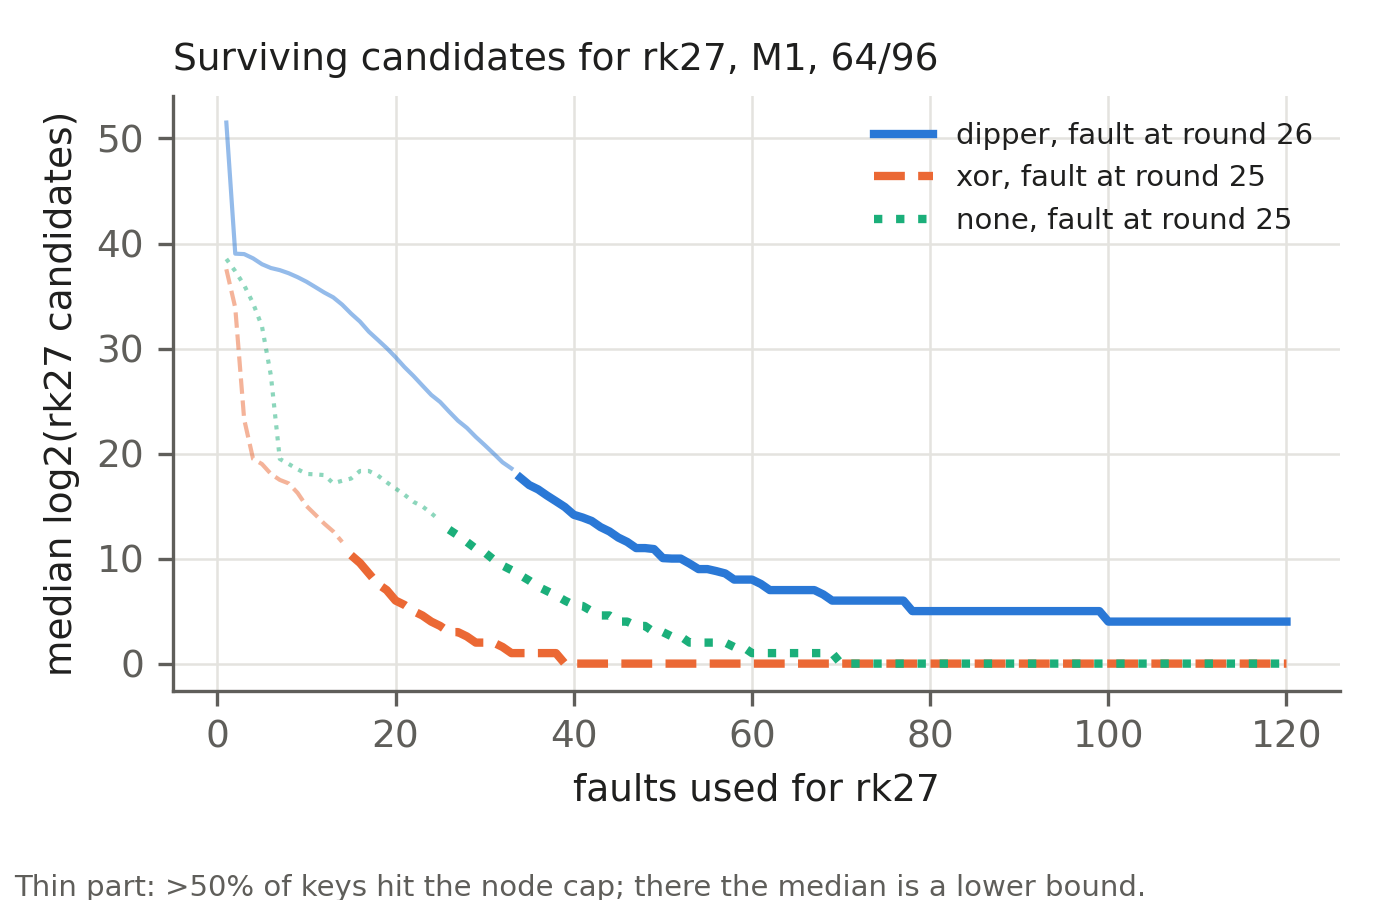
\includegraphics[width=0.62\linewidth]{figures/fig2_survivors.png}
\caption{Median $\log_2$ of the number of surviving $\rk_{27}$ candidates versus the number of
faults, M1, 64/96, 1000 keys. Dipper uses faults in round 26 (near filter); the analysis-only
variants use faults in round 25 (deep filter). In the thin part of each line more than half of
the keys hit the node cap, so the median there is a lower bound.}
\label{fig:surv}
\end{figure}

\subsection{Role of the modular addition}\label{sec:ablation}

Table~\ref{tab:ablation} compares Dipper with the two analysis-only variants for 64/96 under the
floor rule, and Figure~\ref{fig:ecdf} shows the distributions.

\begin{table}[t]
\centering
\caption{Ablation, 64/96, floor rule, 1000 keys per row (same keys and fault streams in each
model). \texttt{xor} and \texttt{none} are analysis-only variants, not proposed as ciphers.
Fault round: $T-1$ = near filter, $T-2$ = deep filter.}
\label{tab:ablation}
\small
\begin{tabular}{lllrrrr}
\toprule
Model & Variant & Fault round & Success & Mean & Median & Max\\
\midrule
M1 & dipper & $T-1$ & 1000 & 225.2 & 210 & 546\\
M1 & xor & $T-1$ & \multicolumn{4}{c}{no information (Prop.~\ref{prop:zero})}\\
M1 & none & $T-1$ & \multicolumn{4}{c}{no information (Prop.~\ref{prop:zero})}\\
M1 & xor & $T-2$ & 1000 & 84.1 & 81 & 184\\
M1 & none & $T-2$ & 1000 & 149.5 & 145 & 278\\
\midrule
M2 & dipper & $T-1$ & 1000 & 126.0 & 115 & 338\\
M2 & xor & $T-1$ & 1000 & 307.9 & 299 & 615\\
M2 & none & $T-1$ & 1000 & 308.2 & 299 & 646\\
\botrule
\end{tabular}
\end{table}

\begin{figure}[t]
\centering
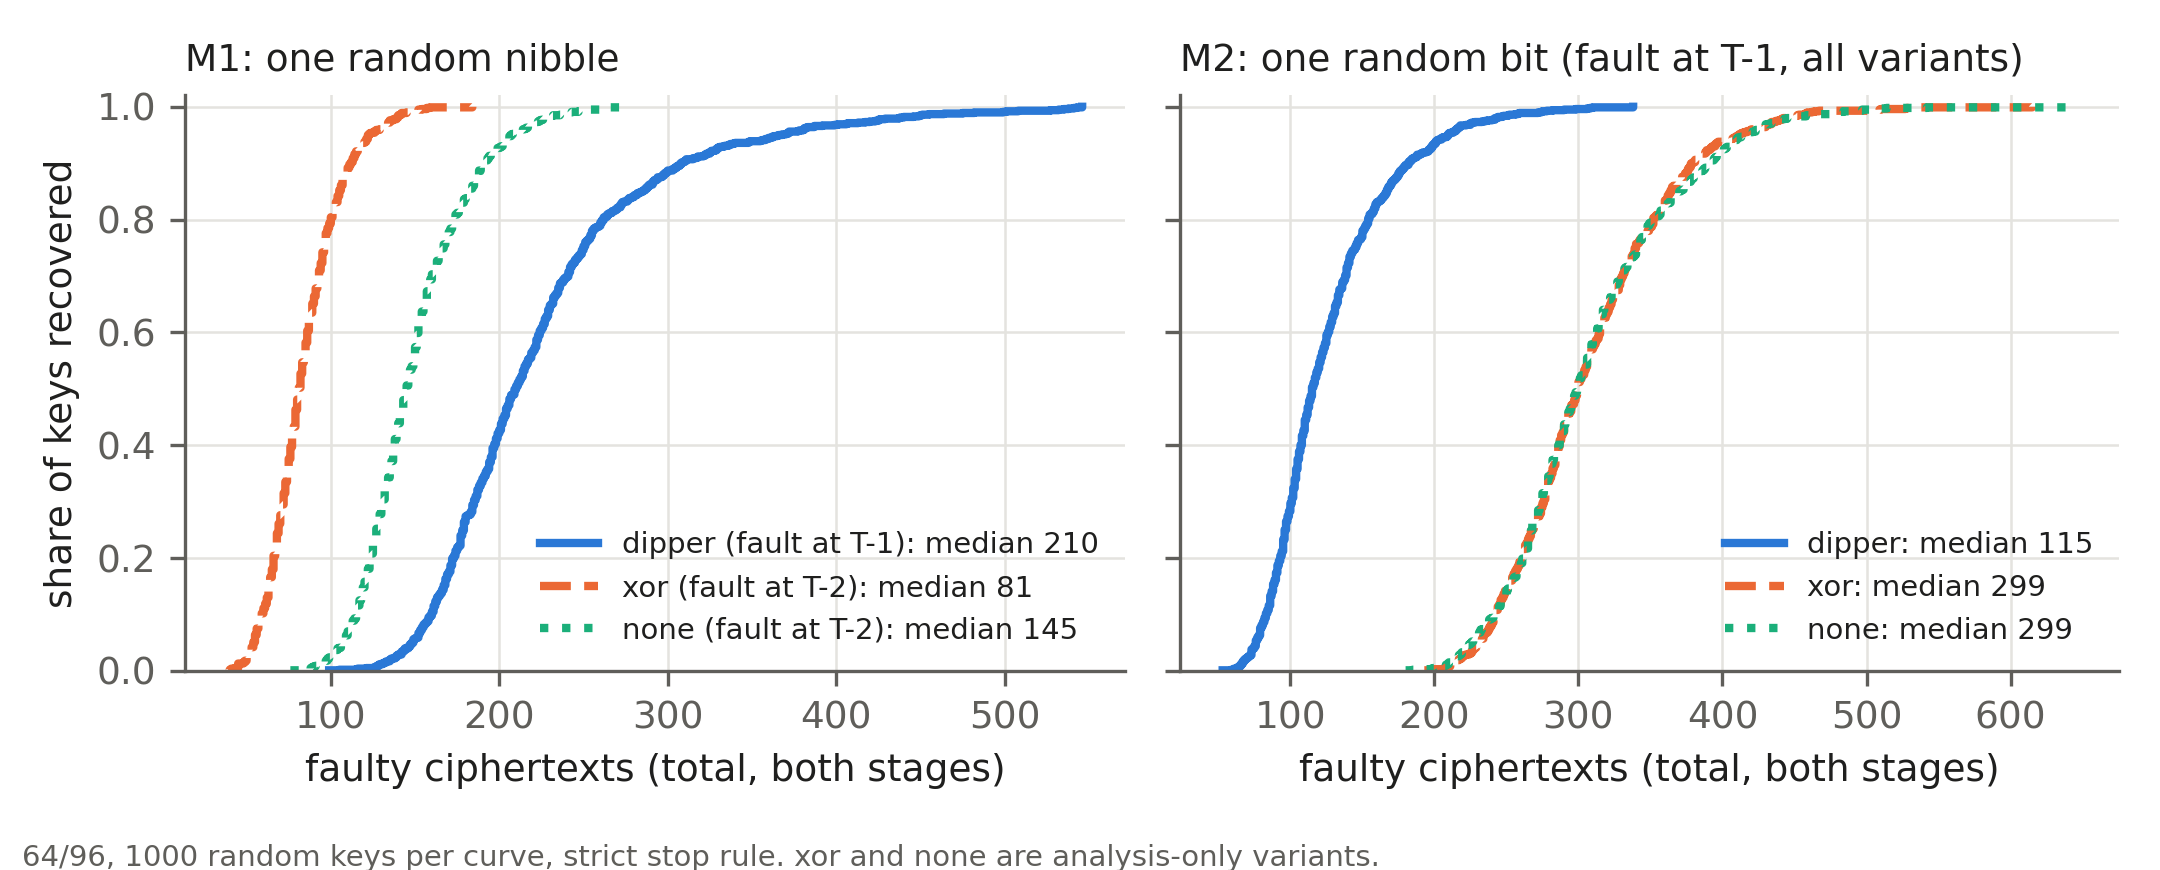
\includegraphics[width=\linewidth]{figures/fig1_faults_ecdf.png}
\caption{Share of keys whose 96-bit master key is recovered after at most $n$ faults (floor
rule, 1000 keys per curve). Left: M1; Dipper with faults one round before each target key,
the variants two rounds before. Right: M2, all variants with faults one round before.}
\label{fig:ecdf}
\end{figure}

Three results stand out.
\begin{enumerate}
\item Under M1 (and M3), the attack used against Dipper gives no information on the variants
without modular addition (Proposition~\ref{prop:zero}). In Dipper, the carries of the
subtraction make the activity pattern at the fault point depend on the key, and this is exactly
what the near filter uses.
\item Under M2, where the same near attack works for all three variants, Dipper needed fewer
faults: median 115 against 299 for both variants.
\item When the variants are attacked with faults one round earlier, they need a median of 81
(\texttt{xor}) and 145 (\texttt{none}) faults under M1, fewer than Dipper with the near filter
(210). This is a different attack, and an equivalent deep attack on Dipper would have to handle
carries in the propagated difference; we did not build it.
\end{enumerate}
In these experiments the modular addition did not raise the cost of DFA. Its main effect was to
give the attacker a key-dependent check one round closer to the ciphertext.

The same pattern holds for 64/128 option A: \texttt{xor} needed a mean of 126.1 faults
(median 123) and \texttt{none} 221.6 (median 215) with the deep filter, against 332.0 (median 316)
for Dipper with the near filter.

\subsection{Secondary fault models}\label{sec:secondary}

Under M2 Dipper needed a mean of 126.0 faults (median 115, max 338) and the filter left a single
master-key candidate. Under M3 with a floor of 8, Dipper needed a mean of 126.7 faults (median
121, max 404), with at most 64 master-key candidates for the final check; with a floor of 4,
265 of 1000 keys did not reach the floor within 1000 faults per stage, which is why the floor of
8 is used. For the variants under M3 the near filter again gives no information, and the deep
filter needed a median of 50 (\texttt{xor}) and 152 (\texttt{none}) faults.

\section{Related work and comparison}\label{sec:related}

We searched the web, IACR ePrint and OpenAlex on 20 October 2026 and found no fault attack on
Dipper; OpenAlex listed no work citing the Dipper paper. Table~\ref{tab:lit} lists published DFA
results for related ciphers. The numbers were taken from the abstracts of these papers. They use
different fault positions, fault models and stop criteria, so they show the order of magnitude
only and are not a direct comparison.

\begin{table}[t]
\centering
\caption{Published DFA results on related ciphers (numbers as stated in the abstracts).}
\label{tab:lit}
\small
\begin{tabular}{p{3.2cm}p{2.0cm}p{4.0cm}p{4.6cm}}
\toprule
Work & Cipher & Fault model & Reported cost\\
\midrule
Xie et al.~\cite{Xie2021} & GIFT-64 & random nibble & master key: 31 faults on average with $2^{16}$ search\\
Luo et al.~\cite{Luo2021} & GIFT & nibble, rounds 25--28 & 64 faulty ciphertexts\\
Bagheri et al.~\cite{Bagheri2013} & PRESENT-80 & single nibble & master key: about 18 faults on average\\
Tupsamudre et al.~\cite{Tupsamudre2014} & SPECK $2n$ & bit flip & last round key: $n/3$ faults on average\\
Huo et al.~\cite{Huo2015} & SPECK & random fault & last round key: about 5--8 faults\\
\midrule
This work & Dipper 64/96 & random nibble (M1) & master key: median 210 (16 left), 116 ($2^8$ left), 91 ($2^{12}$ left)\\
\botrule
\end{tabular}
\end{table}

The GIFT-64 figure of Xie et al.\ (31 faults with a $2^{16}$ search) is lower than ours for
Dipper (median 91 faults with $2^{12}$ candidates left), but the fault positions and stop
criteria differ, and we did not run their attack under our conditions.

\section{Countermeasures}

The attack needs pairs of correct and faulty outputs for the same input. The standard
protection is therefore to detect the fault before the ciphertext is released: compute the
encryption twice (in time or in space) and output the result only if the two agree, or check the
result by decrypting it. These schemes stop the attack described here as long as the fault does
not affect both computations in the same way.

Their main limit is the common-mode fault: when both computations share hardware, code or
data, a single fault can change both in the same way, and the comparison passes. Our related
study~\cite{Huseynli2027} examines which faults in shared resources remain undetected under
duplication-based protection in lightweight block cipher implementations.

A cheaper option is to protect only the last rounds. The attacks measured here used faults in
rounds 24--26 against Dipper (23--25 for the variants with the deep filter), but faults in
earlier rounds were not studied, so we make no claim on how many rounds must be protected. We
did not evaluate any countermeasure experimentally.

\section{Conclusion}

In software simulation, a nibble-fault DFA recovered the full Dipper key in all 1000 trials for
both key sizes, with a median of 210 faulty ciphertexts for 64/96 when 16 master-key candidates
remain and 91 when $2^{12}$ remain, and a median of 208 faults plus a $2^{32}$ search for 64/128.
The modular addition is what makes the round-26 fault informative under nibble and byte faults;
in our measurements it did not increase the number of faults needed compared with variants
without it. We also showed that four bits of each round key cannot be found by this filter under
nibble or byte faults, and that Dipper's last round ends with a keyless, invertible layer, so its
28 rounds amount to 27 keyed nonlinear rounds plus a whitening key.

The study is limited to simulated faults with the stated models and to the attack designed here.
A deep attack on Dipper that handles carries, and experiments with physical fault injection, are
left for future work.

\backmatter

\bmhead{Acknowledgements}
% NOTE (Ali): acknowledgements and the AI-use statement required by the target journal.

\section*{Declarations}

\begin{itemize}
\item \textbf{Funding:} % NOTE (Ali)
Not applicable.
\item \textbf{Competing interests:} The authors declare no competing interests.
\item \textbf{Ethics approval and consent to participate:} Not applicable.
\item \textbf{Consent for publication:} Not applicable.
\item \textbf{Data availability:} Raw results with seeds are available at \url{https://github.com/AlexGuseinov/dipper-dfa}. % NOTE (Ali): create the repository or change the URL.
\item \textbf{Materials availability:} Not applicable.
\item \textbf{Code availability:} The attack, simulation and analysis code is available at the same repository.
\item \textbf{Author contribution:} % NOTE (Ali): fill in.
\end{itemize}

\bibliography{refs}

\end{document}
